\chapter{\IfLanguageName{dutch}{Stand van zaken}{State of the art}}%
\label{ch:stand-van-zaken}

\section{Tekstvereenvoudiging}

Tekstvereenvoudiging is het proces waarin het technisch leesniveau en/of woordgebruik van een geschreven tekst wordt verminderd. Belangrijk hierbij is dat de vereenvoudiging geen effect mag hebben op de kerninhoud. Een complete vereenvoudiging van een tekst bestaat uit minstens drie transformaties \autocite{Siddharthan2014}. Daarnaast is tekstvereenvoudiging een taalbewerking dat geautomatiseerd kan worden. Tekstvereenvoudiging is namelijk een zijtak van natuurlijke taalverwerking.

\subsection{Natural Language Processing}

Natuurlijke taalverwerking of NLP is een brede term die zich richt op het verwerken en analyseren van menselijke taal door computers en andere technologieën. Het omvat verschillende technieken, zoals tekstanalyse, taalherkenning en -generatie, spraakherkenning en -synthese, en semantische analyse. Computers zijn ertoe in staat om op een menselijke manier te communiceren en begrijpen wat er wordt gezegd. Vooraleer het onderzoek zich verdiept in hoe teksten worden vereenvoudigd, moeten er eerst begrippen worden aangehaald die noodzakelijk zijn om de volgende fasen te kunnen uitleggen. \textcite{Sohom2019} haalt de volgende begrippen aan.

\begin{itemize}
	\item \textbf{Tokenisatie} splitst de stam of basisvorm van woorden in een tekst. Gebruikelijk zetten ontwikkelaars deze stap in om een woordenschat voor een taalmodel op te bouwen. Bij tokenisatie wordt er geen rekening gehouden met de betekenis achter ieder woord.
	\item \textbf{Lemmatiseren} in NLP bouwt verder op \textit{stemming}, maar de betekenis van ieder woord wordt in acht genomen. Voor het lemmatiseren bestaan er Nederlandstalige modellen, waaronder JohnSnow\footnote{https://nlp.johnsnowlabs.com/2020/05/03/lemma\_nl.html}. Bij \textbf{omgekeerd lemmatiseren} wordt er een afgeleide achterhaald vanuit de stam. Bijvoorbeeld voor het werkwoord 'zijn' zou dit 'is', 'was' of 'ben' zijn. Voor zelfstandige naamwoorden, zoals 'hond', is dit dan enkelvoud of meervoud.
	\item Bij een \textbf{parsing}-fase wordt er een label aan ieder woord of zinsdeel toegekend. Voorbeelden van labels zijn zelfstandig naamwoord, bijwoord, werkwoord, bijzin of stopwoord. Het herkennen van zinsdelen wordt \textit{chunking} genoemd. Parsing heeft een dubbelzinnigheidsprobleem, want een 'plant' staat niet gelijk aan de vervoeging van werkwoord 'planten'.
\end{itemize}

\subsubsection{Sequence Labeling}

Volgens \textcite{Eisenstein2019} is \textit{sequence labeling} essentieel tot het achterhalen van de structuur van een tekst met \textit{supervised learning}. Elk woord in een tekst of zin wordt geclassificeerd met behulp van specifieke labels, zoals bijvoorbeeld een Part of Speech (PoS) label of een Named Entity Recognition label. De structuur van de tekst wordt achterhaald en informatie en patronen kunnen uit de tekst worden gehaald. 

\section{De verschillende soorten tekstvereenvoudiging}

Tekstvereenvoudiging bestaat uit vier soorten transformaties: lexicale, syntactische en semantische vereenvoudiging en samenvatten.

\begin{figure}
	\begin{center}
			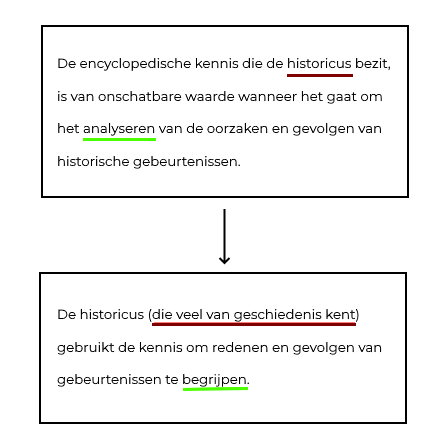
\includegraphics[width=5cm]{img/voorbeeld-manuele-vereenvoudiging.png}
	\end{center}
	\caption{Voorbeeld van manuele tekstvereenvoudiging. Oorspronkelijke tekst uit Historia 5 bron toe te voegen}
\end{figure}

\subsection{Lexicale vereenvoudiging}

% todo bron
Bij lexicale vereenvoudiging worden complexe woorden vervangen door eenvoudigere synoniemen. Bijvoorbeeld, het woord 'adhesief' kan worden vervangen door 'klevend'. De zinsstructuur verandert niet en er is garantie dat de kerninhoud en benadrukking hetzelfde blijft. Het doel van lexicale vereenvoudiging is om de moeilijkheidsgraad van de woordenschat in een zin of tekst te verlagen. Dit is, volgens het aantal onderzoeken, de meest gekende vorm van vereenvoudiging en een noodzakelijke stap bij het vereenvoudigen van een tekst. Voor prevalente domeinen, zoals de onderwijs-, medische en financiële sector, zijn er onderzoeken vrij beschikbaar. 

In de medische sector haalt \textcite{Kandula2010} twee manieren aan om lexicale vereenvoudiging mogelijk te maken, namelijk het vervangen door een synoniem en het aanmaken of genereren van extra uitleg. Zij bouwden verder op een vorig onderzoek van \textcite{Zeng2005}.

\subsection{Syntactische vereenvoudiging}

Syntactische vereenvoudiging transformeert de grammatica en zinsstructuur van een tekst om de complexiteit van een zin te verlagen. Bijvoorbeeld, twee afzonderlijke zinnen kunnen worden samengevoegd tot één eenvoudigere zin. Syntactische vereenvoudiging richt zich op het verminderen van complexe of onduidelijke zinsconstructies, terwijl de inhoud en betekenis van de tekst behouden blijft. Dergelijke transformaties zijn het vereenvoudigen van de syntax of door de zinnen korter te maken. Zinnen worden toegankelijker, zonder de kerninhoud of relevante inhoud te verliezen.

Het vereenvoudigen van medische journalen wordt besproken in het onderzoek van \textcite{Kandula2010}. Zij ontwikkelden een toepassing om medische informatie te vereenvoudigen met beschikbare biomedische bronnen, door syntactische vereenvoudiging op zinniveau toe te passen. Zinnen met meer dan 10 woorden worden als complex beschouwd en worden verwerkt door drie modules. Op het einde van deze vereenvoudiging kan de oorspronkelijke zin ongewijzigd worden behouden of vervangen worden door twee of meer kortere zinnen. De architectuur van het model omvat drie onderdelen: een \textit{Part of Speech (PoS) Tagger}, een \textit{Grammar Simplifier} en een \textit{Output Validator}.

\begin{itemize}
	\item Voor de \textit{PoS Tagger}-fase gebruikten de onderzoekers beschikbare functies uit het open-source pakket OpenNLP\footnote{https://opennlp.apache.org/}.
	\item De \textit{Grammar Simplifier} module splitst de lange zin in twee of meer kortere zinnen door POS-patronen te identificeren en een set transformatieregels toe te passen.
	\item De \textit{Output Validator} module controleert de output van de Grammar Simplifier op grammatica en leesbaarheid. Er zijn drie condities:
	\begin{itemize}
		\item 
	\end{itemize}
\end{itemize}  

% De toepassing werd getest met vier leesbaarheidsmetrieken en een "cloze"-test op verschillende soorten medische documenten, en liet verbeteringen zien in alle metingen. De verbeteringen waren echter relatief klein en er is meer uitgebreide gebruikerstesten nodig voor een betere validatie van het hulpmiddel. De resultaten lieten zien dat het hulpmiddel verbeterd was ten opzichte van eerdere versies. Er is verder werk nodig om de cohesiemeting te verbeteren en de methode voor het genereren van uitleg, waaronder het identificeren van geschikte verbindingswoorden en bronnen voor het genereren van betekenisvolle uitleg.

\subsection{Conceptuele vereenvoudiging}

Conceptuele vereenvoudiging lost dit probleem op. Theoretische kennis hierover is schaars, maar \textcite{Siddharthan2006} bestudeerde dit concept verder. Dit type vereenvoudiging betreft het opdelen van complexe concepten in eenvoudigere delen, het gebruik van duidelijke en bondige taal en het vermijden van technische jargon en abstracte uitdrukkingen. Het doel is om de inhoud begrijpelijker te maken, zonder dat hierbij de betekenis of nauwkeurigheid wordt aangetast. \textcite{Siddharthan2006} noemt deze transformatie een vorm van elaboratie of het uiteenzetten van een begrip.

\subsection{Semantische vereenvoudiging}


\subsection{Tekstvereenvoudiging automatiseren}

Geautomatiseerde tekstvereenvoudiging is niets nieuws. Volgens het onderzoek van \textcite{Canning2000} en \textcite{Siddharthan2006} waren de eerste aanpakken op geautomatiseerde tekstvereenvoudiging gebouwd op rule-based modellen. Deze modellen bewerken de syntax door zinnen te splitsen, te verwijderen of de volgorde van de zinnen in een tekst aan te passen. Lexicale vereenvoudiging kwam hier niet aan de pas. Enkel bij recentere onderzoeken van \textcite{Coster2011} en \textcite{Bulte2018} werd het duidelijk hoe lexicale en syntactische vereenvoudiging gecombineerd kon worden.

\subsection{Combineren tot het geheel van tekstvereenvoudiging}

% Tekstvereenvoudiging omvat drie transformaties. 

Het onderzoek van \textcite{DeBelder2010} richt zich op tekstvereenvoudiging voor kinderen. De doelgroep ligt echter jonger dan deze casus, maar het onderzoek haalt aan hoe de onderzoekers een methode opzetten voor lexicale en syntactische vereenvoudiging.

Een onderzoek van \textcite{Bulte2018} ging met dit concept aan de slag. Het resultaat van hun onderzoek was een \textit{pipeline} ontworpen om moeilijke woordenschat naar simpele synoniemen te vervangen. Eerst ging de tekstinhoud door een \textit{preprocessing}-fase, samen met het uitvoeren van WSE. Daarna werd de moeilijkheidsgraad van ieder token overlopen. De moeilijkheidsgraad is gebaseerd op hoe vaak een woord voorkomt in SONAR500\footnote{https://taalmaterialen.ivdnt.org/download/tstc-sonar-corpus/} een corpus met eenvoudige Nederlandstalige woorden. Synoniemen werden teruggevonden met Cornetto\footnote{https://github.com/emsrc/pycornetto}, een lexicale databank met Nederlandstalige woorden. Hiervoor gebruikten de onderzoekers een \textit{reverse lemmatization} fase. Lexicale vereenvoudiging is ingewikkeld wanneer er geen eenvoudigere synoniemen zijn. In dat geval blijft een moeilijk woord voor wat het is.

\subsection{Samenvatten}

Lexicale, conceptuele en syntactische vereenvoudiging is er geen garantie dat de tekstinhoud korter zal worden. Een langer woord is volgens ... geen indicatief op een complexer woord, zeker wanneer het woord te maken heeft met de opeenvolging van medeklinkers en klinkers.

\textcite{Wafaa2021} deed verder onderzoek op geautomatiseerd samenvatten. Zo zijn er twee verschillende soorten summarization. 

Het onderzoek van \textcite{Hahn2000} bevat vele citaties en is een sterk uitgangspunt om te vertrekken bij samenvatting. Zij halen twee aanpakken hoe een machine een tekst kan samenvatten: extractief en abstractief.

\subsubsection*{Extractief samenvatten}

Bij deze vorm worden de belangrijkste zinnen gemarkeerd en vervolgens opnieuw neergeschreven \textcite{Hahn2000}. Dit is het equivalent van handmatig zinnen te fluoriseren en vervolgens op een blanco papier neerschrijven. 

\textcite{McKeown1999} onderzochten naar de use case voor het extractief samenvatten van teksten. Zij achterhaalden dat deze vorm zeer zwak is voor bias. Bij nieuwsartikelen wordt er geen rekening gehouden met de aanwezige gekantheid van de auteur. De zinnen worden genomen zoals ze zijn.

\textcite{Nallapati2017} wilden de nauwkeurigheid van andere modellen overbruggen. Dit doen ze met \textit{SummaRuNNer}\footnote{https://github.com/hpzhao/SummaRuNNer}, een oplossing voor het extractief samenvatten van teksten met een neuraal netwerk. De toepassing werd opgebouwd met PyTorch in Python en bestaat uit een combinatie van drie modellen: een recurrent neuraal netwerk, een convolutioneel recurrent neuraal netwerk en een \textit{hiërarchical attention network}.

\subsubsection*{Abstractief samenvatten}

Om een abstractieve samenvatting op te bouwen bestaan er verschillende modellen. Het Pegasus-model vloeide voort uit een onderzoek van \textcite{Zhang2020} over het afhandelen van \textit{gap-sentences} met pre-trained models voor samenvatting met NLP. Pegasus haalt kernzinnen uit een invoertekst en zal die zinnen vervolgens als één uitvoerzin uitschrijven. Dit model werd getrained en beoordeeld op samenvattingstaken zoals emails, patenten, rekeningen en ook wetenschappelijke artikelen. Hieronder een code-snippet van hoe een simpele abstractieve samenvatting kan worden gemaakt met Google Pegasus.


\section{Voordelen van tekstvereenvoudiging}

\section{Struikelblokken}

\subsection{Evaluatie van de toepassing}

\subsection{Datasets}

\subsection{Meaning distortion}

\subsection{Word Ambiguity}

Sequence Labeling voorziet labels aan tokens in een tekst. Homoniemen kunnen echter roet in het eten gooien, want . 

\subsection{Paternalisme}
De doelstelling van assisterende software is om gelijke kansen te bieden aan iedereen. Zoals eerder vermeld, zorgt tekstvereenvoudiging voor een simpelere syntax en woordenschat in een tekst. Volgens \textcite{Niemeijer2010} zijn de ethische overwegingen die samenhangen met tekstvereenvoudiging via implicaties voor assistieve technologie niet gemakkelijk te scheiden van de technologie die wordt gebruikt om het resultaat te bereiken. Ontwikkelaars moeten, volgens deze auteur, rekening houden met de doelgroep waarvoor ze een toepassing maken.

Het onderzoek van \textcite{Gooding2022} richtte zich op dit probleem. Ontwikkelaars moeten zich meer bewust worden van de behoeften en verwachtingen van de eindgebruiker bij het ontwikkelen van een tekstvereenvoudigingstoepassing. Haar onderzoek benadrukt de paternalistische en afhankelijke aard van assisterende toepassingen. Tekstvereenvoudiging omvat drie transformaties, maar de moeilijkheidsgraad is niet statisch. Een adaptieve tekstvereenvoudigingstoepassing moet de eindgebruiker een keuze aanbieden om aan te passen wat vereenvoudigd wordt, afhankelijk van zijn of haar specifieke behoeften.

% Xu bron
Volgens \textcite{Punardeep2020}, maken de meeste AI-toepassingen voor tekstvereenvoudiging gebruik van \textit{black-box} modellen. Een \textit{black-box} model maakt het onmogelijk om transparant te zijn over waarom bepaalde transformaties worden uitgevoerd, bijvoorbeeld het vervangen van een woord door een eenvoudiger synoniem. Het model kan dus niet aangeven waarom het juist dat woord heeft vervangen door dat specifieke synoniem. Deze AI-toepassingen vallen onder de categorie van \textit{supervised learning} en het model leert handelingen uit de data waarop het is getraind. Dit is echter problematisch, aangezien \textcite{Xu2015} benadrukt dat veel toepassingen voor tekstvereenvoudiging geen rekening houden met de doelgroep waarvoor ze zijn ontwikkeld.

Om dit probleem op te lossen, is het belangrijk om de eindgebruiker, in dit geval scholieren met dyslexie in het derde graad middelbaar onderwijs, de keuze te geven. Zoals beschreven in \textcite{Gooding2022}, zijn er verschillende mogelijkheden. Bijvoorbeeld, de eindgebruiker moet de mogelijkheid hebben om te kiezen welke synoniemen de tekst lexicaal zullen aanpassen. Een alternatieve aanpak voor syntactische vereenvoudiging is om de scholier zelf zinnen te laten markeren die moeilijk te begrijpen zijn, zodat het systeem alleen de door de eindgebruiker aangegeven zinnen vereenvoudigt.


\subsection{Problemen bij lexicale vereenvoudiging}

\begin{itemize}
	\item Acroniemen
	\item Homoniemen
\end{itemize}

\subsection{Problemen bij syntactische vereenvoudiging}

\begin{itemize}
	\item Kerninhoud verliezen
\end{itemize}

\section{Beschikbare software voor tekstvereenvoudiging}

\subsection{Toepassingen nu in het onderwijs beschikbaar}

\subsection{Online toepassingen}

\section{Pipeline voor tekstvereenvoudiging}

% fasen aanhalen

\subsection{Lexicale vereenvoudiging}

\subsection{Syntactische vereenvoudiging}

\subsection{Samenvatten}

\section{Evaluatiemetrieken}

% Tip: Begin elk hoofdstuk met een paragraaf inleiding die beschrijft hoe
% dit hoofdstuk past binnen het geheel van de bachelorproef. Geef in het
% bijzonder aan wat de link is met het vorige en volgende hoofdstuk.

% Pas na deze inleidende paragraaf komt de eerste sectiehoofding.

% Dit hoofdstuk bevat je literatuurstudie. De inhoud gaat verder op de inleiding, maar zal het onderwerp van de bachelorproef *diepgaand* uitspitten. De bedoeling is dat de lezer na lezing van dit hoofdstuk helemaal op de hoogte is van de huidige stand van zaken (state-of-the-art) in het onderzoeksdomein. Iemand die niet vertrouwd is met het onderwerp, weet nu voldoende om de rest van het verhaal te kunnen volgen, zonder dat die er nog andere informatie moet over opzoeken \autocite{Pollefliet2011}.

% Je verwijst bij elke bewering die je doet, vakterm die je introduceert, enz.\ naar je bronnen. In \LaTeX{} kan dat met het commando \texttt{$\backslash${textcite\{\}}} of \texttt{$\backslash${autocite\{\}}}. Als argument van het commando geef je de ``sleutel'' van een ``record'' in een bibliografische databank in het Bib\LaTeX{}-formaat (een tekstbestand). Als je expliciet naar de auteur verwijst in de zin, gebruik je \texttt{$\backslash${}textcite\{\}}.
% Soms wil je de auteur niet expliciet vernoemen, dan gebruik je \texttt{$\backslash${}autocite\{\}}. In de volgende paragraaf een voorbeeld van elk.

% \textcite{Knuth1998} schreef een van de standaardwerken over sorteer- en zoekalgoritmen. Experten zijn het erover eens dat cloud computing een interessante opportuniteit vormen, zowel voor gebruikers als voor dienstverleners op vlak van informatietechnologie~\autocite{Creeger2009}.
